\chapter{Технологическая часть}

\section{Требования к программе}

К программе предъявляются следующие требования:

\begin{itemize}
	\item программа должна предоставлять пользователю возможность взаимодействовать со слаймом;
	\item оконный интерфейс программы должен предоставлять пользователю возможность изменять такие параметры слайма, как цвет, коэффициент пропускания и показатель поглощения;
	\item должна быть возможность перезагрузки сцены;
\end{itemize}

\section{Выбор инструментов разработки}

Для выполнения данной работы был выбран высокоуровневый язык
программирования C++. Данный выбор обусловлен следующими факторами:

\begin{itemize}
	\item C++ поддерживает технологию объектно-ориентированного
	программирования, которая позволяет легко модифицировать программу и
	эффективно организовывать взаимодействия между объектами;
	\item С++ обладает очень высокими показателями вычислительной
	производительности, что также обеспечивает достойную скорость исполнения
	кода;
	\item для C++ было создано множество библиотек, которые могут быть
	использованы, в частности, для математических расчетов.
\end{itemize}

В качестве среды разработки была выбрана Visual Studio Code по
следующим причинам:

\begin{itemize}
	\item данная среда разработки бесплатна;
	\item в данной среде присутствуют встроенный отладчик, инструменты для
	работы с Git и средства навигации по коду, автодополнения кода и контекстной
	подсказки;
	\item имеется возможность расширить любой функционал, включая
	компиляцию и отладку.
\end{itemize}

Для создания графического пользовательского интерфейса был выбран фреймворк QT. Данный выбор обуславливается быстрой многоуровневой разработкой интерфейса и наличием классов для работы с изображениями. Соответственно, для сборки проекта была выбрана утилита qmake.

Для параллелизации работы алгоритма обратной трассировки лучей и вычисления векторов сил и новых координат точек масс моделируемого объекта была выбрана библиотека pthread. Данный выбор обуславливается возможностью создания потоков в соответствии со стандартом POSIX, который позволяет разрабатывать переносимые программы.

\section{Диаграмма классов}

На рисунке \ref{uml} изображена диаграмма классов, использующихся в программе.

\begin{figure}[h!]
	\centering
	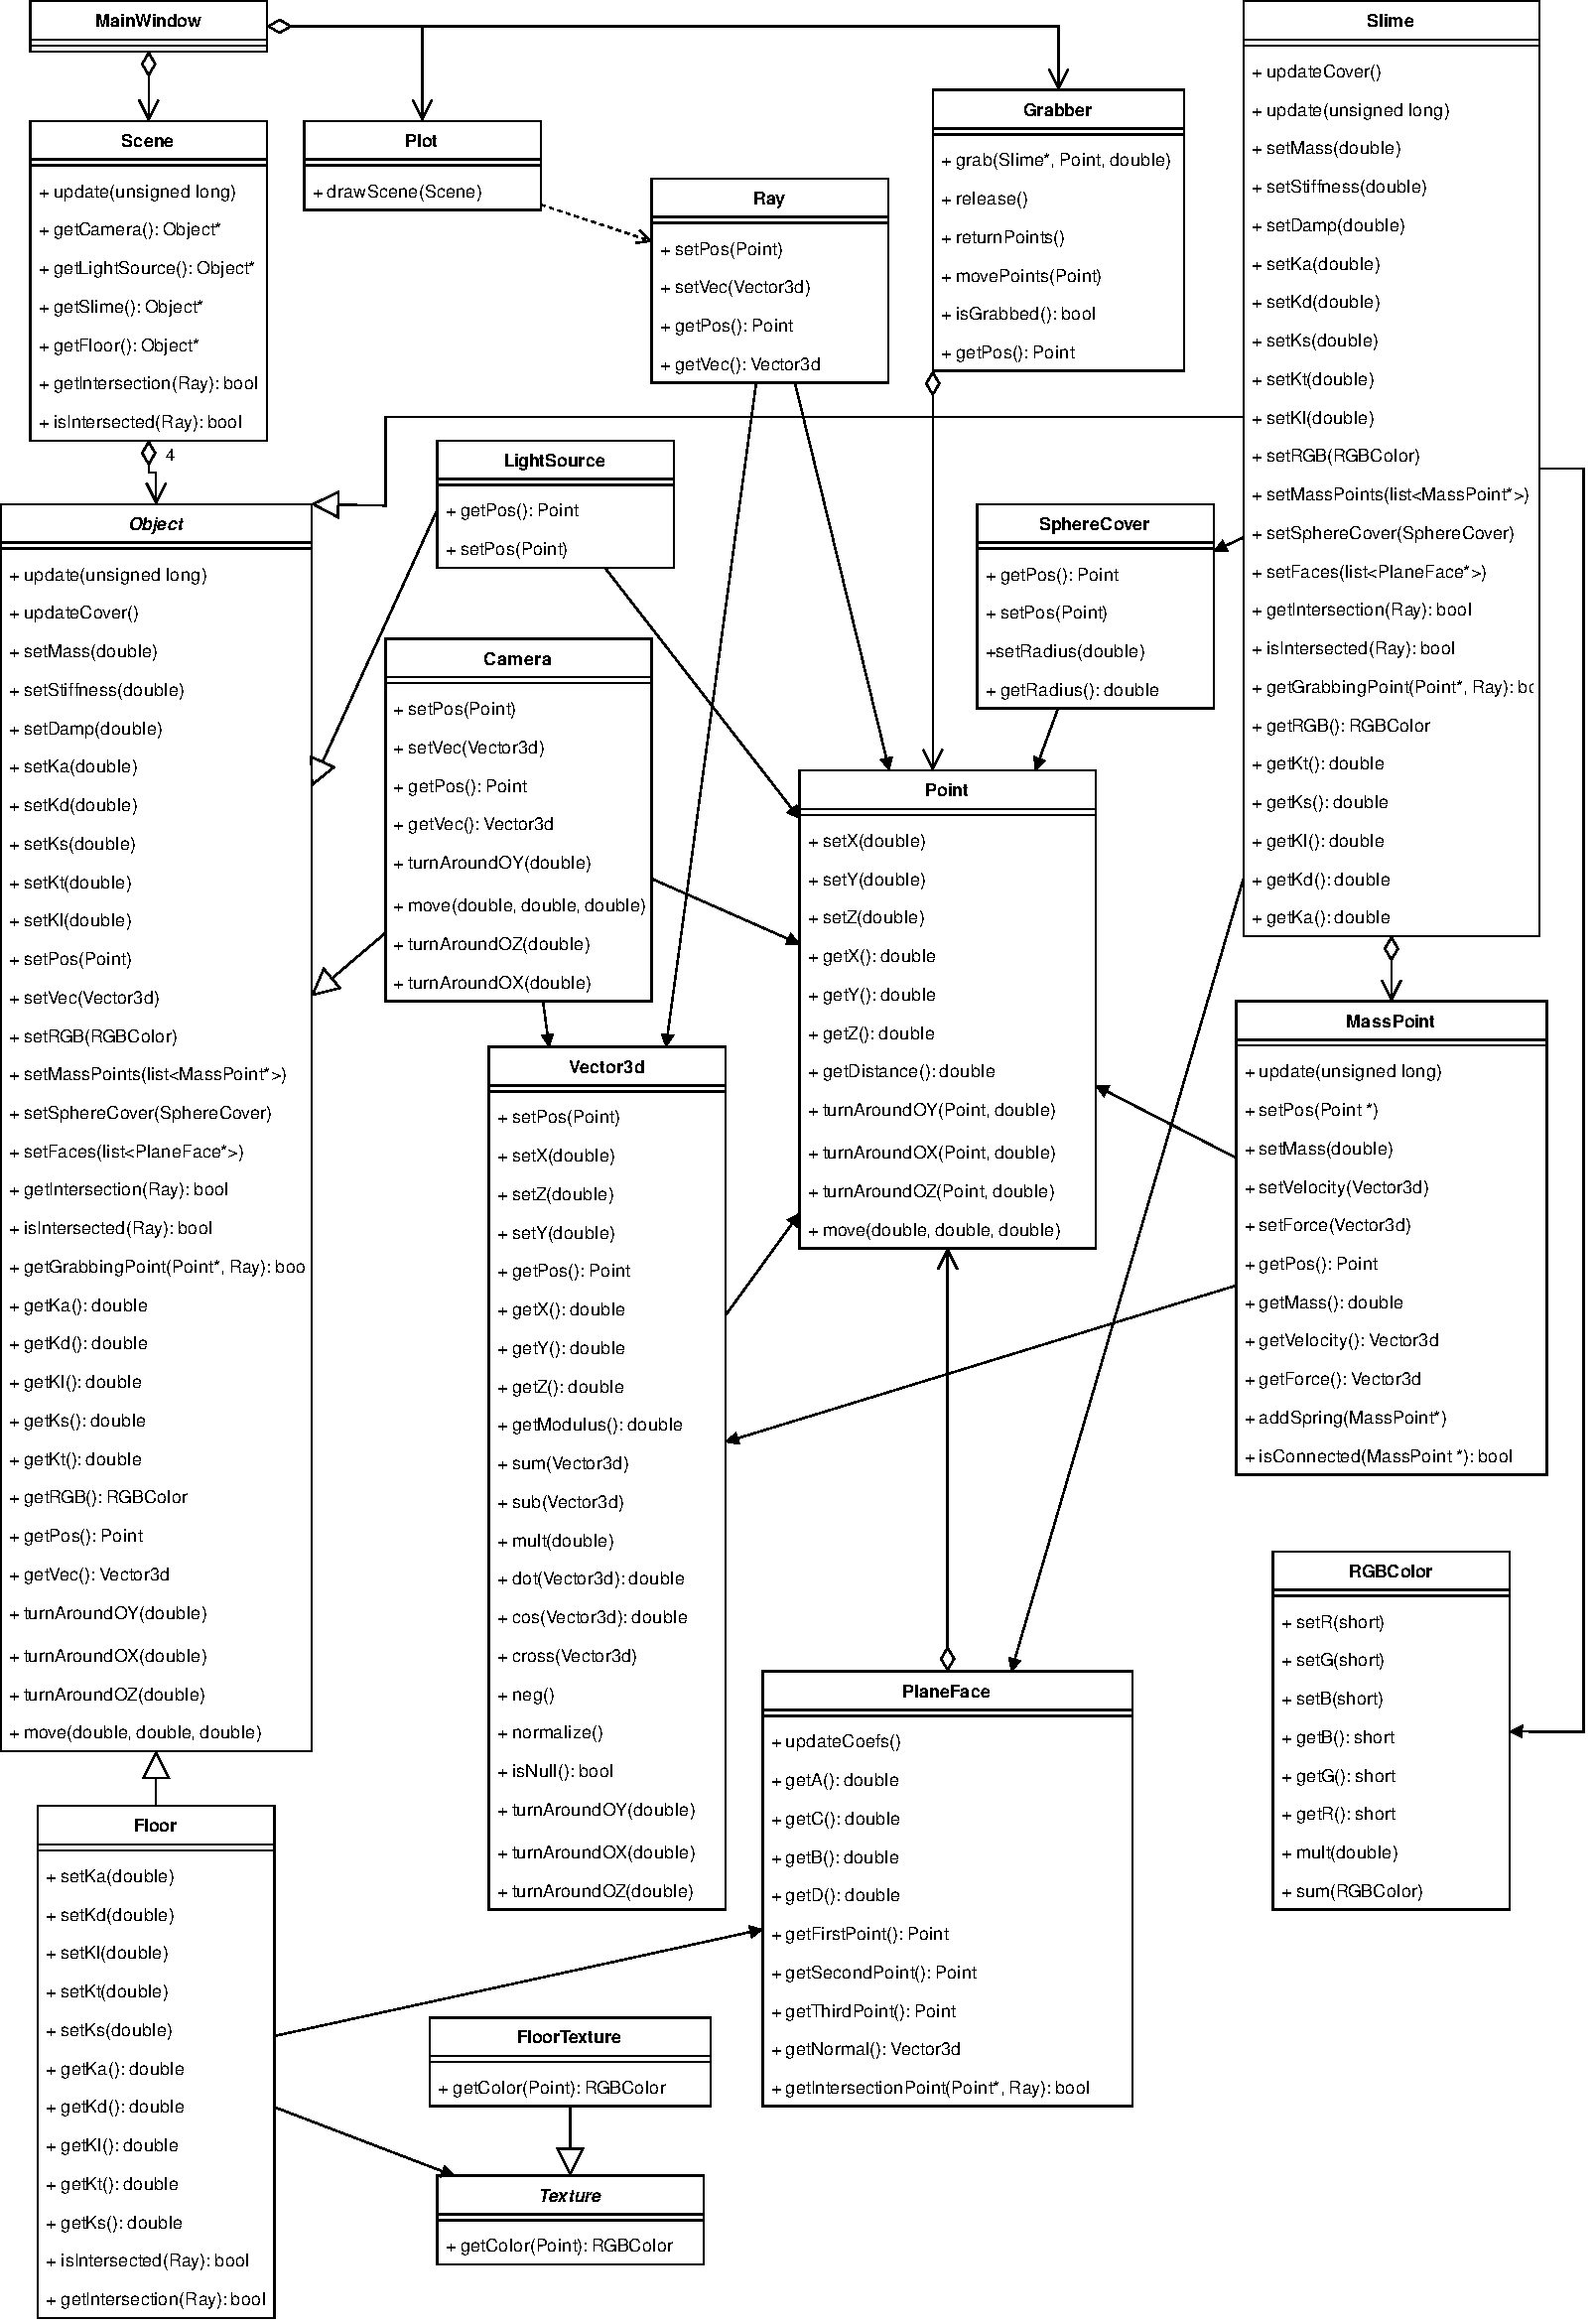
\includegraphics[width=\linewidth]{uml}
	\caption{Диаграмма классов}
	\label{uml}
\end{figure}

В программе используются следующие абстракции:

\begin{itemize}
	\item MainWindow --- класс оконного интерфейса;
	\item Scene --- класс, хранящий в себе информацию об объектах сцены;
	\item Plot --- класс, использующийся для визуализации сцены;
	\item Grabber --- класс, хранящий информацию о захваченной пользователем вершине слайма;
	\item Object --- абстрактный класс объекта сцены;
	\item Camera --- класс, хранящий информацию о камере;
	\item LightSource --- класс точечного источника света;
	\item Floor --- класс пола;
	\item Slime --- класс слайма;
	\item Point --- класс геометрической точки;
	\item Vector3d --- класс трехмерного вектора;
	\item MassPoint --- класс точки массы;
	\item RGBColor --- класс, хранящий информацию о цвете в схеме RGB;
	\item PlaneFace --- класс плоской треугольной грани;
	\item SphereCover --- класс сферической объемлющей оболочки слайма;
	\item Texture --- абстрактный класс текстуры объекта;
	\item FloorTexture --- класс текстуры пола;
	\item Ray - класс луча.
\end{itemize}

\section{Интерфейс программы}

На рисунке \ref{ui} показан интерфейс программы.

\begin{figure}[H]
	\centering
	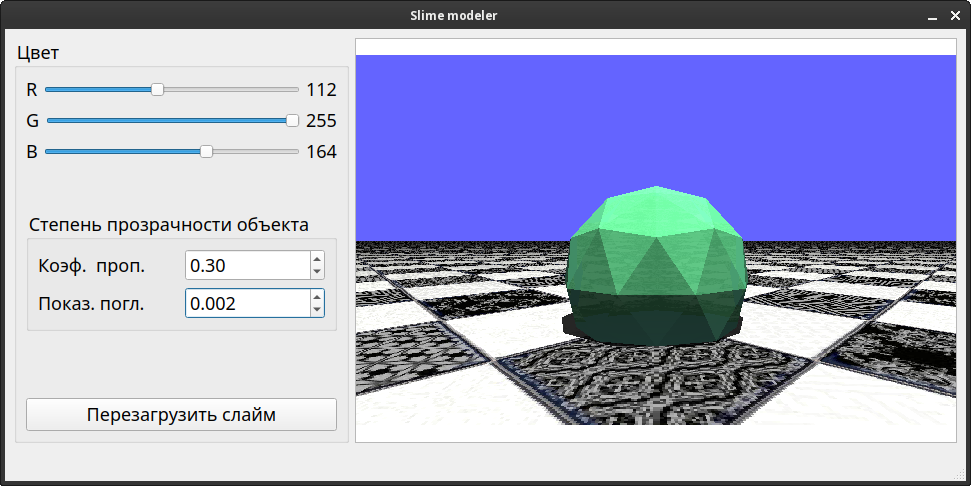
\includegraphics[width=\linewidth]{ui}
	\caption{Интерфейс программы}
	\label{ui}
\end{figure}

Цвет слайма устанавливается с помощью трех слайдеров, отвечающих за красный, зеленый и синий компоненты цветовой модели RGB соответственно. Степень прозрачности устанавливается двумя полями для ввода вещественных чисел, отвечающих за коэффициент пропускания и показатель поглощения слайма. Кнопка <<Перезагрузить слайм>> используется для перезагрузки сцены.

\section*{Вывод}

В данном разделе были выбраны инструменты для разработки программного обеспечения. Были созданы графический пользовательский интерфейс и диаграмма классов.

\clearpage
